\section{Introduction}
\label{sec:intro}

\todo[inline]{Motivation and overview.}

Things we need to do somewhere in this paper:
\begin{itemize}
	\item Convince everyone that this is awesome. It would be particularly cool if we can somehow make the case that these ideas are relevant even if people aren't doing stack based work. Can we do that, though? Most (i.e., tree-based)
	GP systems don't allow for things like silencing of nodes or replacing nodes
	with NOOPs because it typically wouldn't be clear how to interpret such a tree.
	\item Cover relevant work. This might require some digging?
	\item Cover relevant background. This is going to (at least) require explaining PLUSH genomes, the conversion from PLUSH to PUSH, the evaluation of PUSH programs (so we can understand what NOOPs do), and silent genes.
	\item Describe the 5 simplification methods
	\item Experimental setup
	\item Results
	\item Discussion
	\item Future work
	\item Conclude
\end{itemize}

Smaller solutions have other benefits as well: understandability, faster runtimes, etc. But, we won't concentrate on those in this paper.

Automatic simplification was introduced to Push as a tool for making evolved programs easier to understand \cite{Robinson:2001:GPtieus, spector:2002:GPEM}. While it can be applied to any program, it has typically been used post-run to make solution programs easier to understand without changing their behavior \cite{Spector:2014:GECCOcomp}. It has also been used as a bloat-control genetic operator during genetic programming runs, with mixed success \cite{Zhan:2014:GECCOcomp}. \todo[inline]{Does this paragraph belong here in the intro or in the Simplification section?}
\todo[inline]{I'd say here in the intro. -- Nic}

\section{PUSH, PLUSH, etc.}
\label{sec:push}

\todo[inline]{Explain necessary aspects of PUSH, PLUSH, and the like. Include talk of silencing genes, and how a silenced gene does not affect the resulting program, including instructions and closing parentheses.}

\todo[inline]{We should briefly define what the ``size'' of a push program is, since we discuss size a lot later.}

\todo[inline]{Need to define error vector somewhere.}

\section{Automatic Simplification in Push}
\label{sec:simplification}

Automatic simplification is a simple hill-climbing algorithm that tries to make an individual's program smaller without changing the program's behavior on the training cases. At each step, we first make small changes to the program to make it smaller. We then check whether the smaller program produces the same error vector as the original program. If so, we continue with the new program; 
otherwise, we revert to the previous program. This process repeats for a set 
number of simplification steps, and then returns the resulting simplified program. The algorithm is presented in detail in Algorithm \ref{alg:simplification}.

\begin{algorithm}[t]
\caption{Automatic Simplification}
\label{alg:simplification}

\SetKwInOut{Input}{Input}
\SetKwData{ErrorVector}{errorVector}
\SetKwData{NewErrorVector}{newErrorVector}
\SetKwData{Ind}{ind}
\SetKwData{NewInd}{newInd}
\SetKwData{Steps}{steps}
\SetKwData{S}{s}
\SetKwFunction{ComputeErrors}{computeErrorVector}
\SetKwFunction{TakeStep}{takeSimplificationStep}

\Input{individual \Ind, number of simplification \Steps, method for simplification step \TakeStep}
\BlankLine

\ErrorVector $\leftarrow$ \ComputeErrors{\Ind} \;
\For{\S $\leftarrow 0$ \KwTo \Steps}{

	\NewInd $\leftarrow$ \TakeStep{\Ind} \;
	\NewErrorVector $\leftarrow$ \ComputeErrors{\NewInd} \;
	\If{\NewErrorVector $=$ \ErrorVector}{
		\Ind $\leftarrow$ \NewInd
	}
}
\Return \Ind
\end{algorithm}

In this paper we explore five different methods of automatic simplification. Each method follows the same general algorithm; they only differ in the particular steps taken to make programs smaller. %The five methods are listed in Table ???, along with a description of what they do at each simplification step.
Below is a description of each method:

\textbf{Program} simplification, which has been used in Push since its inception \cite{Robinson:2001:GPtieus}, acts on an individual's Push program, as opposed to its linear Plush genome. At each simplification step, it has an 80\% chance of removing one or two random ``code points'' from the program, where a \textit{code point} is an instruction, a constant, or a parenthesized block of code. The other 20\% of the time it randomly removes one set of parentheses from a code block in the program, flattening the code inside the parentheses into the level that the code block occupied.

The other four simplification methods act on an individual's linear Plush genome prior to its translation into a Push program. There are three basic steps that are used across these genome methods: silencing random genes, unsilencing random genes, and NOOPing random genes. Silencing a gene activates its ``silent'' epigenetic marker, making that instruction not appear the resulting Push program, 
as well as not opening any new parenthesized code blocks or ending any open parenthesized code blocks. When picking a random gene to silence, we never select a gene that is already silent.

Note that by silencing genes instead of removing them entirely, it 
becomes possible to backtrack by unsilencing previously silenced genes. 
Thus, in several methods 
we silence some genes while unsilencing others, making it possible to 
backtrack by activating genes that were previously turned off. We hope that the backtracking enabled by unsilencing will allow simplification to escape some local program size minima that it might otherwise be impossible to escape, resulting in more reliable simplification to smaller programs. Similar to silencing, we never select an unsilenced gene to unsilence. 

Finally, some methods ``NOOP'' genes by replacing their instructions with 
NOOP instructions that have no effect when executed. 
Some Push programs require an instruction to be present in a location, 
with no particular concern for that instruction's details. It is not
uncommon, for example, for programs to use the number of instructions on
the \texttt{exec} stack as a counter or a numeric constant, but without ever
actually executing those instructions. 
We can replace these instructions with NOOPs without affecting the semantics
of the program, potentially making the program more general without actually 
making it smaller, or possibly enabling further simplifications. 
Genes that are already NOOPed cannot be selected by a NOOP step of 
simplification.

\begin{table}[t]
	\centering
	\caption{Genome simplification methods. Each method lists the possible single simplification steps it can take during simplification, and the probability of taking each step.}
	\label{table:genome-methods}
	\begin{tabu} to \textwidth {l l r}
		\toprule
		\textbf{Method} & \textbf{Step} & \textbf{Prob.}  \\
		\midrule
		\textbf{Genome} & Silence 1 (gene) & 0.50 \\
		       & Silence 2 & 0.30 \\
		       & Silence 3 & 0.10 \\
		       & Silence 4 & 0.10 \\
		\midrule
		\textbf{Genome-Backtracking}
		       & Silence 1 & 0.40 \\
		       & Silence 2 & 0.25 \\
		       & Silence 3 & 0.10 \\
		       & Silence 4 & 0.05 \\
		       & Silence 1, Unsilence 1 & 0.05 \\
		       & Silence 2, Unsilence 1 & 0.10 \\
		       & Silence 3, Unsilence 1 & 0.05 \\
		\midrule
		\textbf{Genome-Noop}
		       & Silence 1 & 0.40 \\
		       & Silence 2 & 0.25 \\
		       & Silence 3 & 0.10 \\
		       & Silence 4 & 0.05 \\
		       & Noop 1 & 0.10 \\
		       & Noop 2 & 0.10 \\
		\midrule
		\textbf{Genome-Backtracking-}
		       & Silence 1 & 0.30 \\
		  \textbf{Noop} & Silence 2 & 0.20 \\
		       & Silence 3 & 0.10 \\
		       & Silence 1, Unsilence 1 & 0.05 \\
		       & Silence 2, Unsilence 1 & 0.10 \\
		       & Silence 3, Unsilence 1 & 0.05 \\
		       & Noop 1 & 0.10 \\
		       & Noop 2 & 0.10 \\
		\bottomrule
	\end{tabu}
\end{table}

The four genome methods of simplification are listed in Table \ref{table:genome-methods}. Each method lists the types of steps that can be taken and the probability of each step being chosen. The most basic of the methods, 
\textbf{Genome} simplification only allows for the silencing 
of 1 to 4 random genes in a single step. \textbf{Genome-Backtracking} and \textbf{Genome-Backtracking-Noop} occasionally unsilence a silent gene while silencing another, allowing the process to not follow a strict hill-climbing scheme.  \textbf{Genome-Noop} and Genome-Backtracking-Noop use NOOPing to turn intructions into NOOPs without removing them entirely.

Note that while the Program simplification method can remove unnecessary parentheses from a program, none of the genome methods have this ability. Since the genome methods change the genomes themselves, which have no parentheses, they cannot remove the parentheses that appear in the resulting translated program. They can silence an entire gene, which will omit its instruction and any open parentheses it requires, but they cannot simply remove a pair of extraneous parentheses.

\section{Experimental setup}
\label{sec:setup}

In our experiments, we wanted to answer several key questions. 
First, does automatic simplification effectively improve the generalization of evolved programs that pass every training case? 
Further, which of the simplication methods described in the previous section 
produces the smallest programs, which generalizes the best, and is there correlation between getting smaller and generalizing better?

To examine these questions, we conducted simplification experiments using evolved solution programs from a suite of general program synthesis benchmark problems \cite{Helmuth:2015:GECCO}. This benchmark suite is composed of 29 general programming problems taken from introductory computer science course homework assignments. These problems require solution programs to utilize a wide range of programming constructs, such as multiple data types, control flow structures, and multiple inputs/outputs.
After the original publication of these benchmark problems \cite{Helmuth:2015:GECCO}, they have seen use in a range of studies using PushGP (eg. \cite{Helmuth:2016:GECCO, McPhee:2016:GPTP, Helmuth:2015:GPTP, Helmuth:2015:dissertation}),  % TMH: could potentially remove 1 or 2 of these if we need the space
as well as recent work considering a general program synthesis grammar for 
grammar guided genetic programming \cite{Forstenlechner:2017:eurogp}.

For these problems, we are primarily interested in whether we can find a program that passes every training case and unseen test case, since programs that do not achieve such perfection do not represent true solutions to the problems \cite{Helmuth:2015:GECCO}. We will call a program that passes all of the training set a ``solution'', and a program that additionally passes all of the unseen test set a ``generalizing solution''.

We took our evolved solution programs from the original set of benchmarking runs using the benchmark suite \cite{Helmuth:2015:GECCO}. In those original
runs, each problem was attempted 100 times each for several selection methods;
in this work, we only use the 100 runs that used lexicase selection, as it
consistently had the highest success rates and provided solutions to the most problems. 
In these runs, PushGP created at least one generalizing solution to 22 of the problems. In addition, we include one problem (Super Anagrams) for which 14 programs were evolved that passed the training set but did not pass the unseen test set. We also include the Checksum problem, which was not solved in the runs for the original publication, but was subsequently solved with some additions to the training set.

In earlier work, it was shown that simplifying the same program many times can result in a range of resulting program sizes \cite{Spector:2014:GECCOcomp}. To acount for this variance in the simplified programs, we performed multiple simplifications of each solution program. For each of our five simplification methods, we conducted 100 separate simplification trials of each solution program, recording the size and generalization of each simplified program. 
Some of the original, unsimplified programs also entirely passed the 
unseen test set (i.e. generalized), and some did not (i.e. did not generalize). When running GP on real-world problems, one will not know whether an evolved solution program generalizes or not before using simplification. Thus we are interested in not only what happens to evolved programs that do not generalize, but also to those that already generalize. For example, it would not be beneficial to improve generalization of some programs while reducing generalization of many more programs.

For each simplification trial, we simplified the solution program using 10,000 steps of the simplification algorithm (see Algorithm~\ref{alg:simplification}). 
While this number of steps is often more than necessary to effectively 
simplify most programs, the simplification process is not prohibitively expensive. Note that while every simplification step requires evaluating the new program, making 10,000 simplification steps moderately expensive, this is the equivalent number of evaluations to 10 generations of GP with a population of 1000. Since we are advocating for simplification at the end of a GP run, it only needs to happen once, 
so expending this much computational effort seems reasonable.

The benchmark suite we used prescribes using randomly generated training and test cases for most of the input and output data. Since automatic simplification requires use of training data, we use the training and test sets that were used for the original run for every simplification of the solution program from that run.



\section{Results}
\label{sec:results}

\begin{figure*}[t] %[t] sets the image at the top of the page; t = top, b = bottom, h = here%
\centering
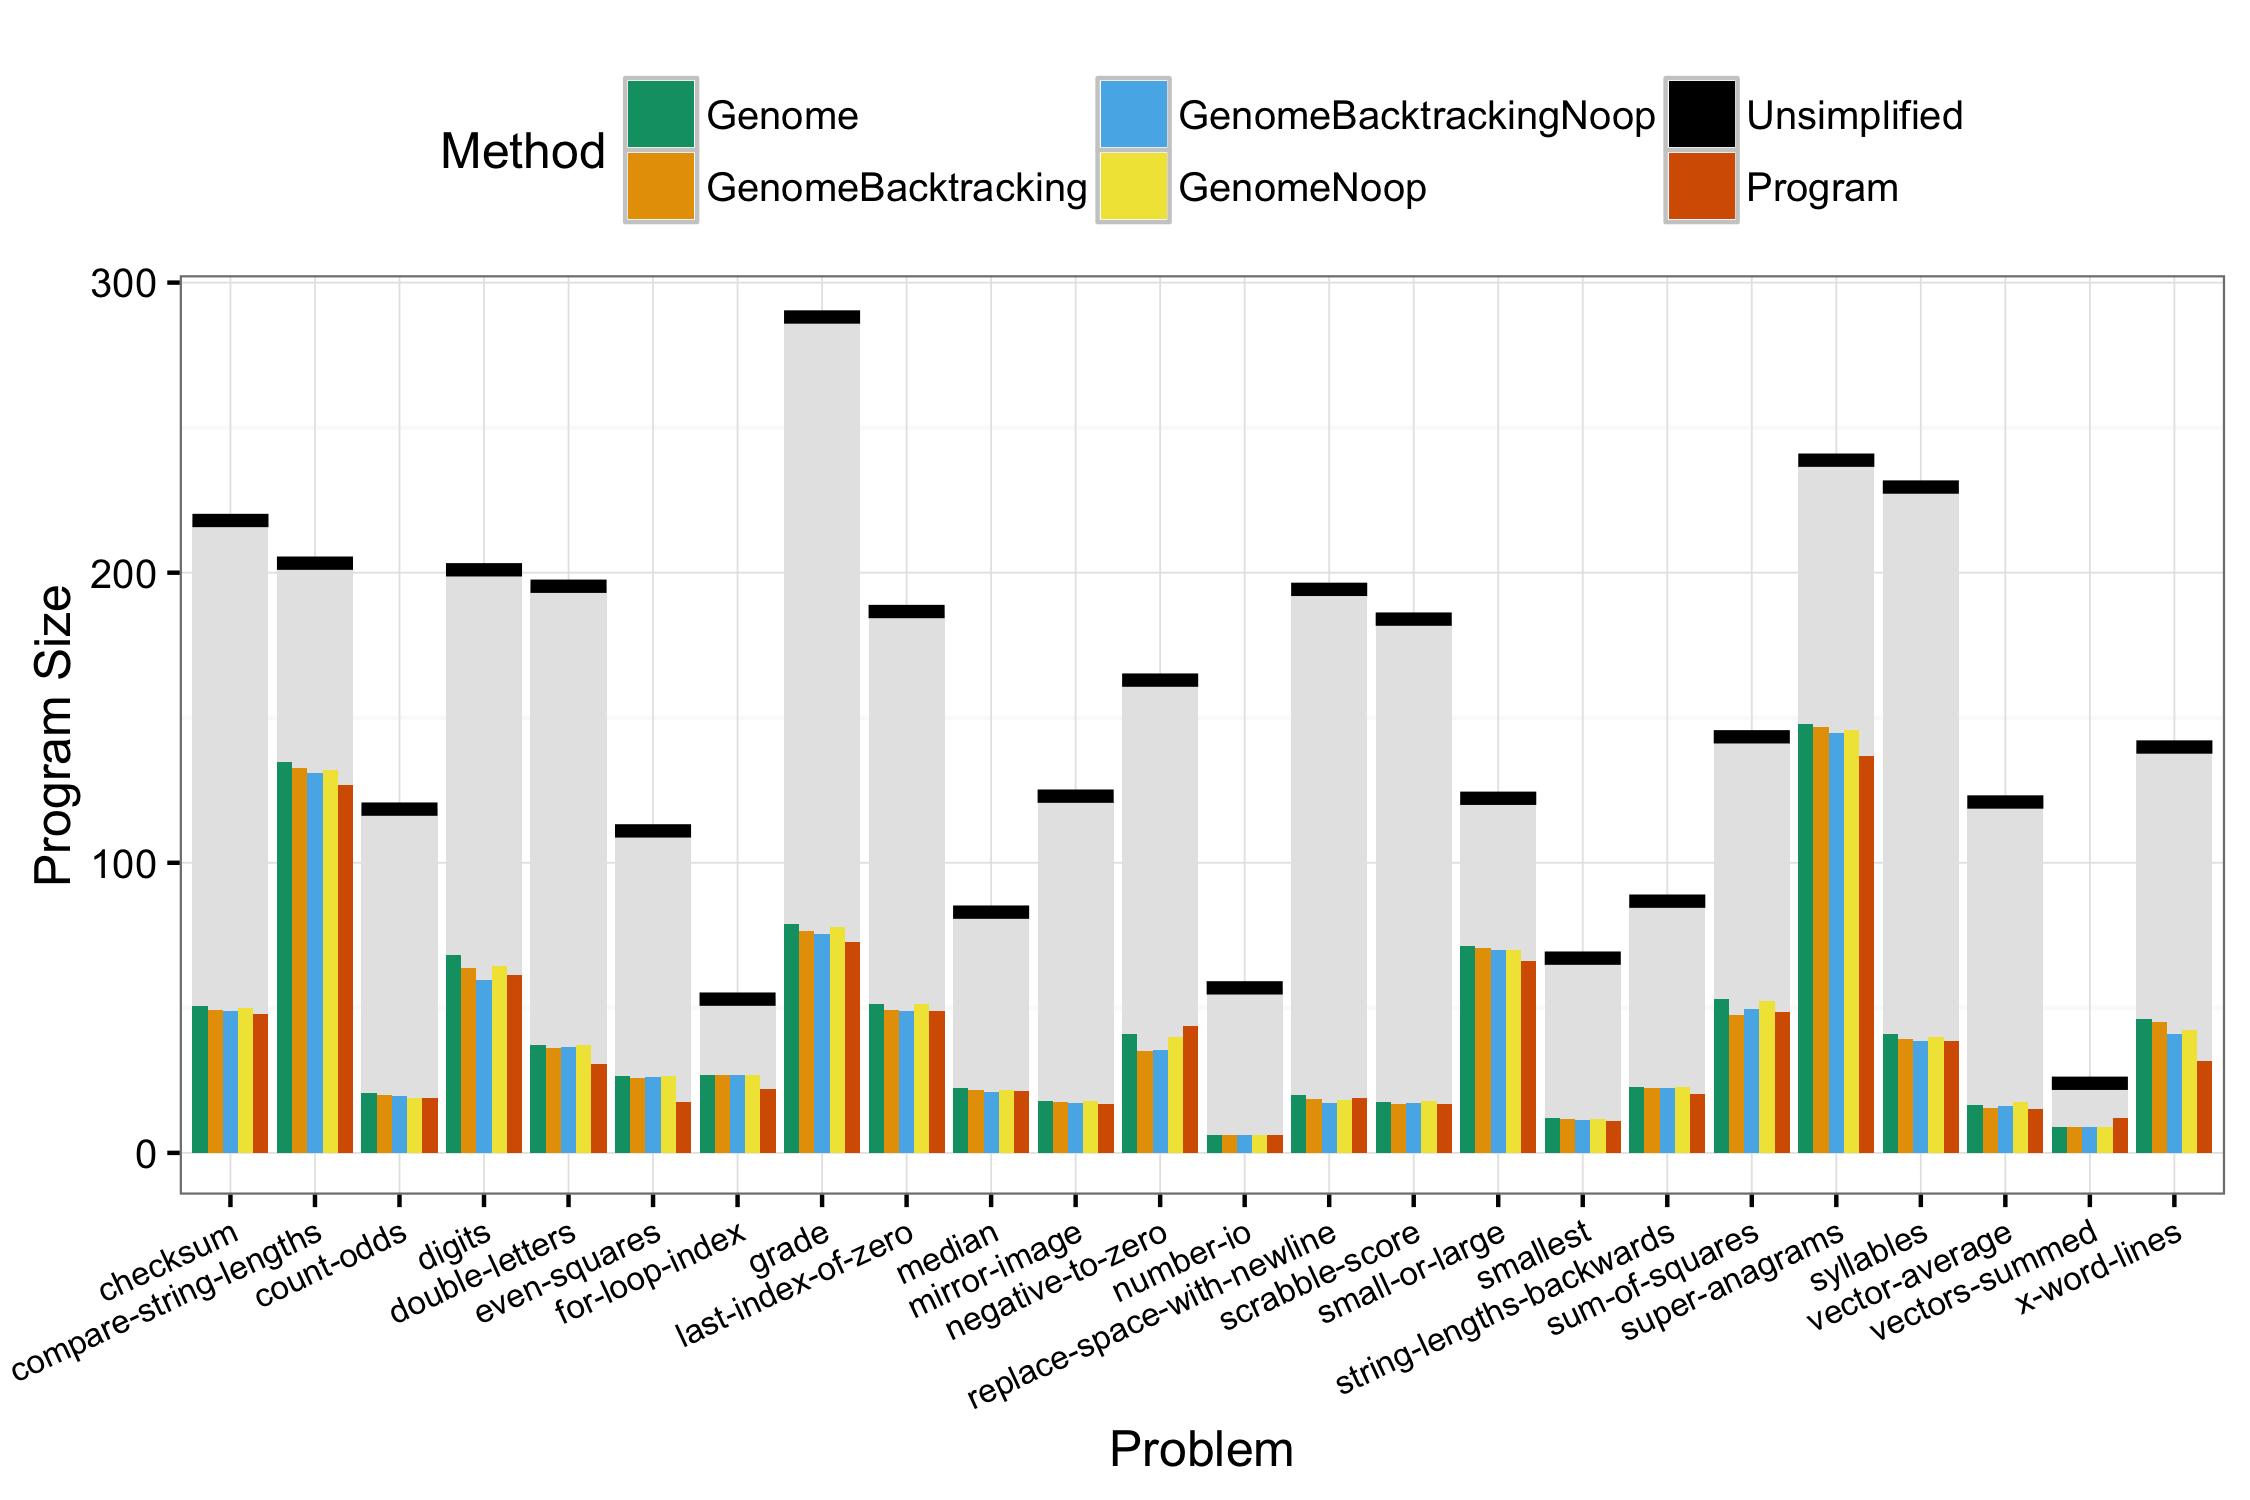
\includegraphics[width=0.95\textwidth]{Problem_by_Size_bar} % \linewidth
\caption{The average program size of programs produced by our five 
	simplification methods for each problem set; the average program 
	sizes of the unchanged programs are represented with black 
	horizontal bars. Each simplification method performs repeated trials 
	using the same set of unchanged programs, and therefore has 
	the same opportunities for simplification as the other methods. }
\label{fig:bar:size}
\end{figure*}

%\hl{Question: Should we somehow indicate the number of data points that go into each problem? Some problems have a lot of unchanged solutions ($>$ 90), and some have very few ($<$ 10), with the latter group potentially being small sample size, and the former group having more effect on the aggregate plots across problems.}
%\todo[inline]{It took me a while to figure out the question, but the 
%	later comment about DL only having 6 solutions to work with caused the 
%	light bulb to go off. I suspect we should indicate this somewhere. A table 
%	would be big. Maybe putting the number of initial successes in parens after 
%	the problem name in the axis labels? -- Nic}

We first consider the question of how much effect simplification has on the size of each solution program. Figure~\ref{fig:bar:size} presents the average program size of the unchanged solution programs on each problem as a horizontal black line. It then gives the average simplified size of the simplified solution programs, with 100 trials per solution, for each of our five simplification methods. It is immediately clear that every simplification method has a large impact on the average size of the solution programs, with most shrinking to half their original size or smaller. 
In fact, the size
differences resulting from the various simplification methods are all 
quite small when compared to the difference between the simplified sizes
and the unchanged programs' sizes.

\begin{table}[tb]
	\centering
	\caption{The average rank in size for each simplification method across the data in Figure~\ref{fig:bar:size}, where lower rank means smaller programs. ``Unchanged'' is the rank of the evolved programs without any simplification. Methods are sorted by average rank.}
	\label{table:size-ranks}
	\begin{tabu} to \textwidth {l r}
		\toprule
		\textbf{Method} & \textbf{Average Rank} \\
		\midrule
		\textbf{Program} & 1.87 \\
		\textbf{Genome-Backtracking-Noop} & 2.13 \\
		\textbf{Genome-Backtracking} & 2.79 \\
		\textbf{Genome-Noop} & 3.60 \\
		\textbf{Genome} & 4.60 \\
		\textbf{Unchanged} & 6.00 \\
		\bottomrule
	\end{tabu}
\end{table}

To examine aggregate performance of each simplification method, in Table~\ref{table:size-ranks} we calculate the average rank for size for each method across the 24 problems, with rank 1 indicating the smallest average program size and rank 6 having largest. Note that we include the unchanged programs as one ``method'', which is why we have 6 possible ranks. Program simplification achieves the smallest programs on average, with both of the Genome backtracking methods coming soon after. The genome methods without backtracking have worse average ranks, with the unchanged programs always having worst rank. Since parentheses are counted as part of the size of a program, and since the Genome methods cannot remove extraneous parentheses as mentioned in Section~\ref{sec:simplification}, we hypothesize that Program simplification is able to achieve smaller sizes largely based on removing such parentheses.

The Friedman test on the data in Table~\ref{table:size-ranks} gives a \textit{p}-value $< 0.001$, indicating that at least one method performs significantly differently from the others. We then use a post-hoc Wilcoxon-Nemenyi-McDonald-Thompson test \cite{hollander1999nonparametric} to give the significance in the differences in ranking between each pair of methods at the $0.05$ significance level. Every simplification method besides Genome outranks the Unchanged programs. Program also outranks Genome-Noop and Genome; and both Genome backtracking methods outrank Genome. Note that even though these results show significant differences in rank among the methods, most of the actual differences in average size are relatively small compared to the sizes of the unchanged programs.

%Program - none                              3.685940e-14
%GenomeBacktrackingNoop - none               6.733392e-12
%GenomeBacktracking - none                   1.343098e-08
%Program - Genome                            4.483262e-06
%GenomeBacktrackingNoop - Genome             4.216509e-05
%GenomeNoop - none                           9.320840e-05
%GenomeBacktracking - Genome                 8.811779e-03
%Program - GenomeNoop                        1.506233e-02
%---------------------------------------------------------
%  Cutoff for p-value of 0.05 or less (above)
%---------------------------------------------------------
%GenomeNoop - GenomeBacktrackingNoop         6.179964e-02
%Genome - none                               9.284012e-02
%GenomeNoop - Genome                         4.175994e-01
%Program - GenomeBacktracking                5.190458e-01
%GenomeNoop - GenomeBacktracking             6.489706e-01
%GenomeBacktrackingNoop - GenomeBacktracking 8.119145e-01
%Program - GenomeBacktrackingNoop            9.971909e-01

Next, we consider the effect of simplification on the generalization of programs to unseen test data. In Figure~\ref{fig:bar:percent_generalization}, we plot the percent of programs that generalize for each simplification method, as well as a horizontal bar representing the percent of unsimplified programs that generalize.

\begin{figure*}[t] %[t] sets the image at the top of the page; t = top, b = bottom, h = here%
\centering
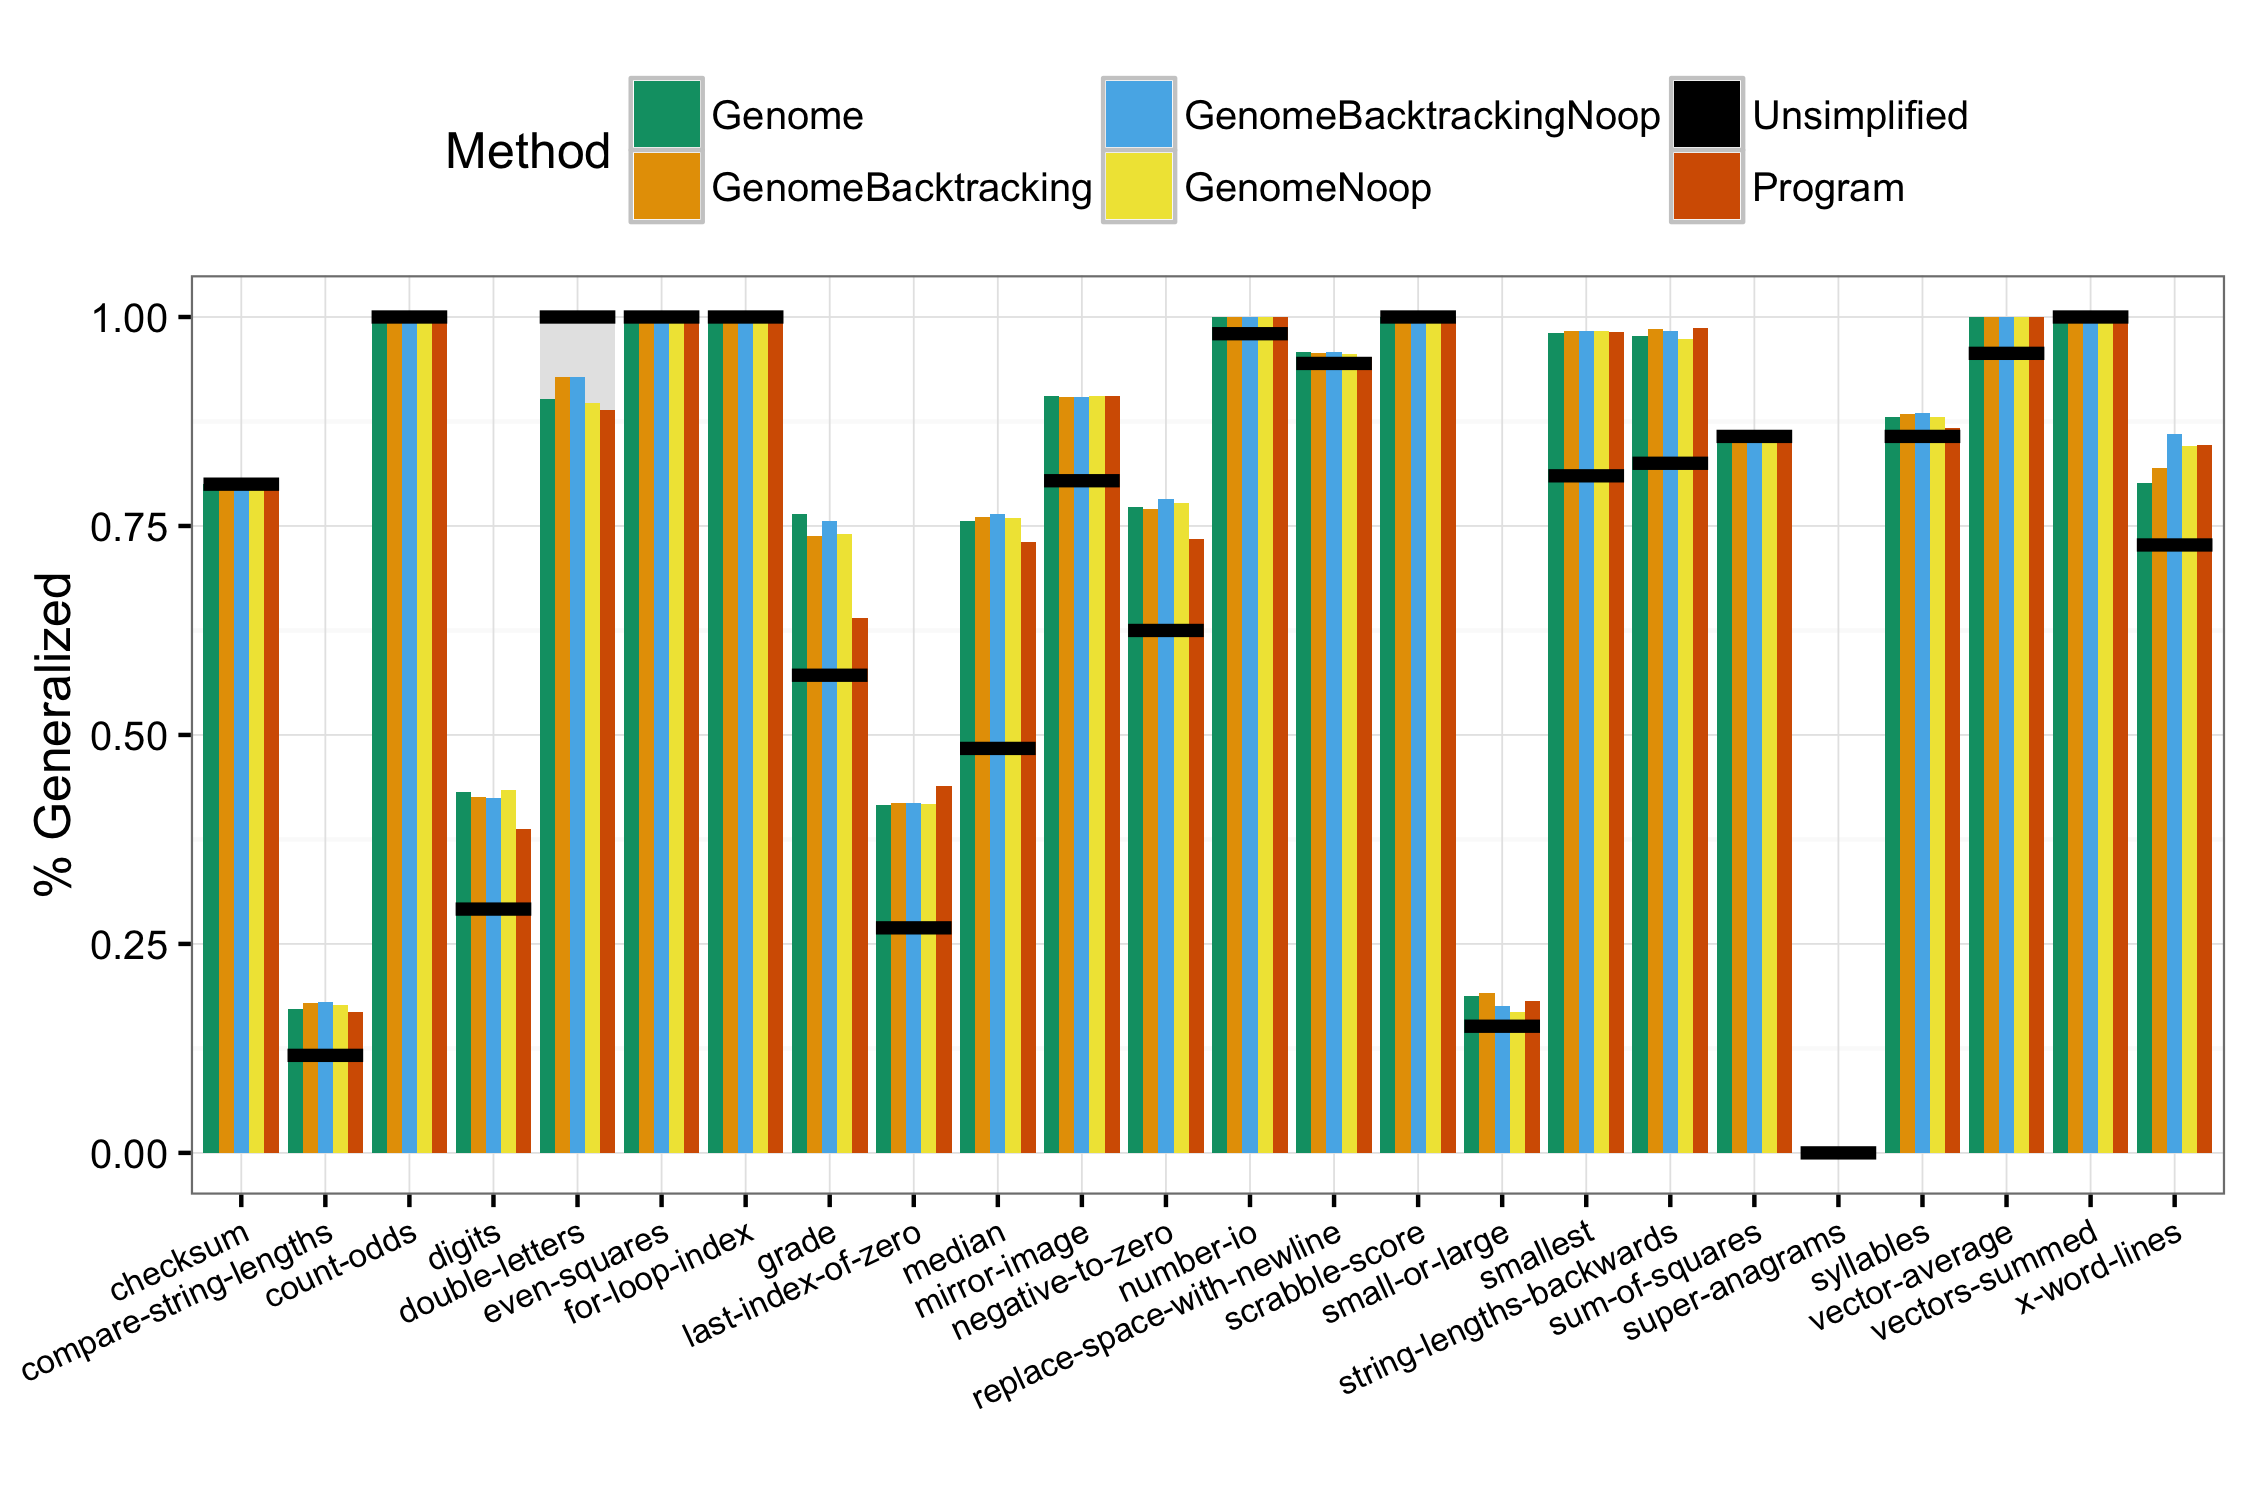
\includegraphics[width=0.95\textwidth]{Problem_by_PcntGen_bar} % \linewidth
\caption{The proportion of simplified programs that generalize to unseen data
	for each problem, with the proportion of unchanged programs that generalize 
	indicated with black horizontal bars.
 \hl{Question: In this figure, how much of the time are the simplified programs significantly better at generalization than the unsimplified programs? How would we measure this? Do we need to?}}
 \hl{Is this just a bunch of \texttt{prop.test} in R, or am I not understanding
 	the question?}
\label{fig:bar:percent_generalization}
\end{figure*}

Every simplification method either improves generalization or has no effect on every problem besides Double Letters.\footnote{The Double Letters problem has one of the smaller sample sizes of our data set, with only six solution programs as starting points. All six solutions generalize before simplification. Five of the six generalize most of the time after simplification, but one solution program has many simplifications that don't generalize.} Some of the increases in generalization appear substantial, 
improving as much as 25\% in the case of the Median problem.

Also note that the five problems with the worst generalization in Figure~\ref{fig:bar:percent_generalization} are among the problems for which program sizes were largest in Figure~\ref{fig:bar:size}. For whatever reason, programs that solve these problems tend to be large and unable to shrink, and do not generalize well. We hypothesize, but have no data to support, that large programs such as these contain many ad-hoc components that overfit to individual test cases without really ``learning'' the underlying program structure, and therefore do not generalize to unseen data.

%This supports our hypothesis that programs that are smaller but behaviorally identical on the training set tend to generalize better.

As with average program sizes, there do not appear to be large differences between the simplification methods in terms of generalization. To see if the small differences do affect rank, we calculated the average rank of each method across all problems. Here, rank 1 signifies the best (highest) generalization, and rank 6 represents the worst generalization. These average ranks are presented in Table~\ref{table:generalization-ranks}.

\begin{table}[ht]
	\centering
	\caption{The average rank in generalization for each simplification method across the problems in Figure~\ref{fig:bar:percent_generalization}, where lower rank means better generalization. ``Unchanged'' is the rank of the evolved programs without any simplification. Methods are sorted by average rank.}
	\label{table:generalization-ranks}
	\begin{tabu} to \textwidth {l r}
		\toprule
		\textbf{Method} & \textbf{Average Rank} \\
		\midrule
		\textbf{Genome-Backtracking-Noop} & 2.73 \\
		\textbf{Genome-Backtracking} & 3.02 \\
		\textbf{Genome-Noop} & 3.29 \\
		\textbf{Genome} & 3.33 \\
		\textbf{Program} & 3.67 \\
		\textbf{Unchanged} & 4.96 \\
		\bottomrule
	\end{tabu}
\end{table}

For generalization, the differences in rank for the simplification methods are not as pronounced as with simplified sizes. Note that Program simplification, while producing the smallest programs, has the worst generalization of the simplification methods; all of the Genome-based methods remain in the same order. The Friedman test on the data in Table~\ref{table:generalization-ranks} gives a \textit{p}-value $< 0.001$, indicating that at least one method performs significantly differently from the others. We then use a post-hoc Wilcoxon-Nemenyi-McDonald-Thompson test \cite{hollander1999nonparametric} to give the significance in the differences in ranking between each pair of methods at the $0.05$ significance level. Here, every simplification method significantly outranks Unchanged. But, there is not a significant difference in generalization rank between any of the simplification methods. Thus the average rank of each method is approximately the same, which is unsurprising considering their similarities in Figure~\ref{fig:bar:percent_generalization}.

%GenomeBacktrackingNoop - none               1.532704e-06
%GenomeBacktracking - none                   8.164085e-05
%GenomeNoop - none                           1.186298e-03
%Genome - none                               1.892900e-03
%Program - none                              2.829973e-02
%%---------------------------------------------------------
%%  Cutoff for p-value of 0.05 or less (above)
%%---------------------------------------------------------
%Program - GenomeBacktrackingNoop            2.338544e-01
%Program - GenomeBacktracking                6.504160e-01
%GenomeNoop - GenomeBacktrackingNoop         7.712306e-01
%GenomeBacktrackingNoop - Genome             7.129661e-01
%GenomeBacktracking - Genome                 9.774709e-01
%GenomeNoop - Genome                         9.999987e-01
%Program - Genome                            9.701077e-01
%GenomeBacktrackingNoop - GenomeBacktracking 9.834383e-01
%GenomeNoop - GenomeBacktracking             9.881573e-01
%Program - GenomeNoop                        9.505945e-01


\begin{table}[t]
	\centering
	\caption{This table records every single simplified program across all problems. The top row corresponds to unchanged programs that did not generalize, where the bottom row is those that did generalize. The left column contains all simplified programs that did not generalize, and the right column has those that did. For example, we see that there are 53787 simplified programs that generalize coming from original programs that did not generalize.}
	\label{table:total-counts}
	\begin{tabu} to \textwidth {l r r}
		\toprule
		& \multicolumn{2}{p{2.8cm}}{\textbf{Generalizes \newline Post-Simplification}} \\
		& \textbf{No} & \textbf{Yes} \\
		\midrule
		\textbf{Generalizes Pre: No} & 102617 & 53787 \\
		\textbf{Generalizes Pre: Yes} & 3735  & 289265 \\
		\bottomrule
	\end{tabu}
\end{table}

Table~\ref{table:total-counts} presents the total count of each combination of programs that did/did not generalize pre-simplification with did/did not generalize post-simplification. Considering the first row, we see that of the evolved programs that did not generalize, over one third generalized after simplification. This is a large increase in generalization. On the other hand, out of the starting programs that did generalize before simplification (the second row), only about 1.2\% of the simplifications broke them so that they did not generalize. This gives strong evidence that simplification can be used to make evolved programs more likely to generalize, without a large risk of breaking programs that already generalize.

\begin{figure}[t] %[t] sets the image at the top of the page; t = top, b = bottom, h = here%
\centering
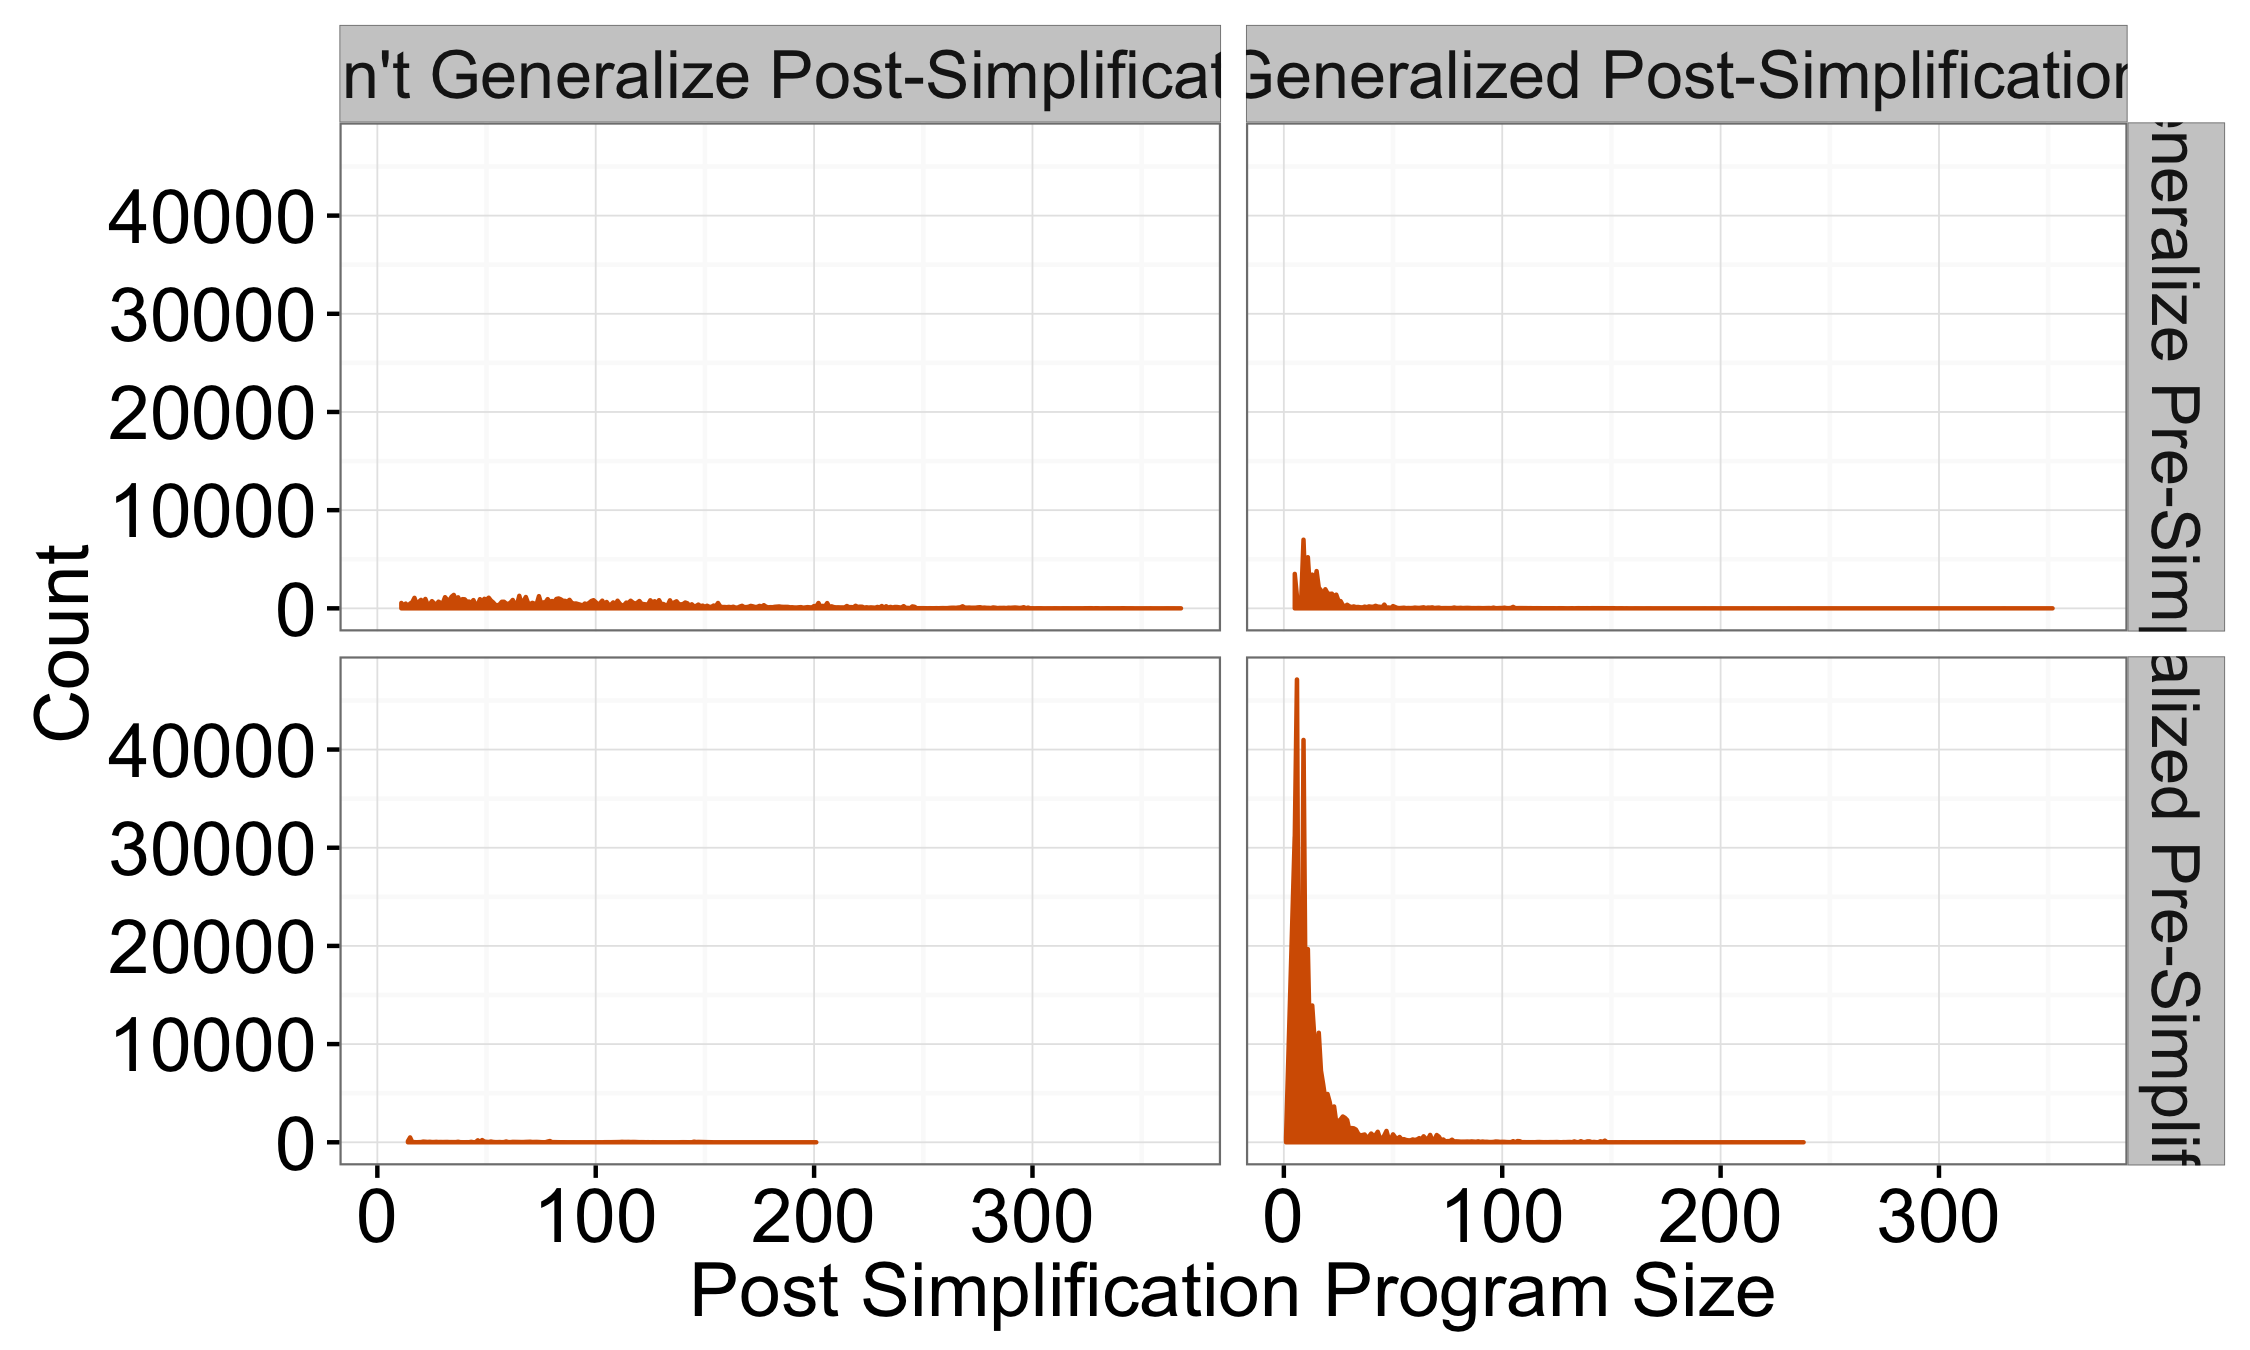
\includegraphics[width=\linewidth]{Quad_Density}
\caption{\hl{needs caption}}
\label{fig:count:quad}
\end{figure}

%\begin{figure}[t] %[t] sets the image at the top of the page; t = top, b = bottom, h = here%
%\centering
%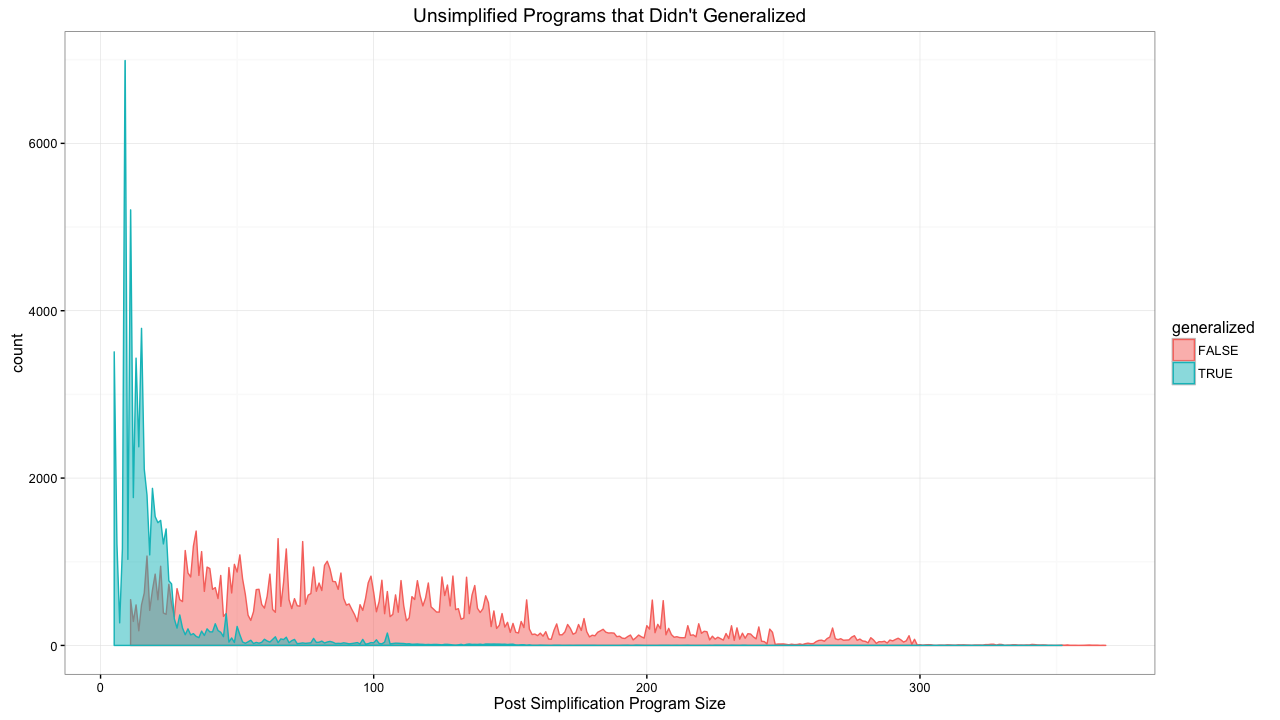
\includegraphics[width=\linewidth]{Size_density_by_generalized_B_no_facet_count}
%\caption{Size counts of simplified programs where pre-simplified program did \underline{not} generalize.}
%\label{fig:count:pre-simp-gen-false}
%\end{figure}
%
%\begin{figure}[t] %[t] sets the image at the top of the page; t = top, b = bottom, h = here%
%\centering
%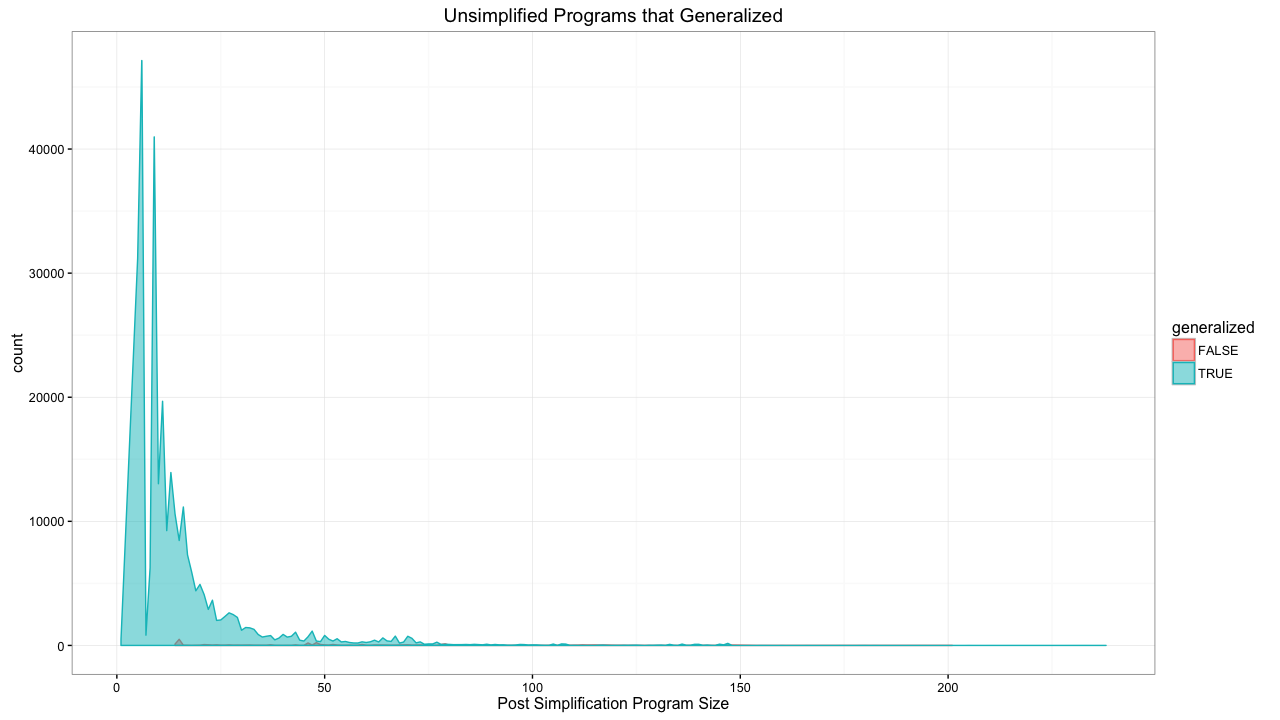
\includegraphics[width=\linewidth]{Size_density_by_generalized_A_no_facet_count}
%\caption{Size counts of simplified programs where pre-simplified program did generalize.}
%\label{fig:count:pre-simp-gen-true}
%\end{figure}

\hl{Note:} I just replaced 2 figures with the quad-figure in Figure \ref{fig:count:quad}. The next two paragraphs will need some rewriting, but the gist will be the same.

We next want to explore how size after simplification corresponds to the generalization of simplified programs. Figures~\ref{fig:count:pre-simp-gen-false} and \ref{fig:count:pre-simp-gen-true} each plot the counts of the sizes of the simplified programs for different sets of programs, aggregated across all problems. Figure~\ref{fig:count:pre-simp-gen-false} only includes those simplifications that started with unchanged programs that did not generalize. This figure clearly shows that when the resulting simplified program was relatively small (with size less than about 25), it was much more likely to change from ungeneralizing to generalizing (shown by the blue line). On the other hand, programs that remained larger after simplification were more likely to not have their generalization affected by simplification (shown by the red line). Thus, most of the improvements in generalization that we described previously come from simplified programs that achieve small sizes. This clearly shows that there is a correlation, if not causation, between post-simplification size and the probability of generalization.

Figure~\ref{fig:count:pre-simp-gen-true} gives the same counts of sizes of the simplified programs, but this time for those unchanged programs that did generalize. First, note that the scale of the $y$-axis is over 5 times as large as for Figure~\ref{fig:count:pre-simp-gen-false}; this tells us that many more of the unchanged programs did generalize (\hl{is this true???}). Here, we are interested in whether many of the unchanged programs that did generalize were broken by simplification to the point of not generalizing. We see that very few such instances occured compared to those that remained generalizing after simplification. Thus while simplification often makes a program go from ungeneralizing to generalizing, it does not often take a generalizing program and make it ungeneralizing.

The correlation between post-simplification size and generalization can also be seen in Figure~\ref{fig:nic-plot}. Here, each point represents one simplified program; which plot it belongs to depends on whether it generalized before or after simplification. The $x$-axis gives pre-simplification size of the program, and the $y$-axis gives simplified program size; thus, every point must lie under the $y = x$ line. Points close to the $y = x$ line did not reduce much during simplification; those further below the $y = x$ line correspond to those that shrank more.

\begin{figure}[t] %[t] sets the image at the top of the page; t = top, b = bottom, h = here%
\centering
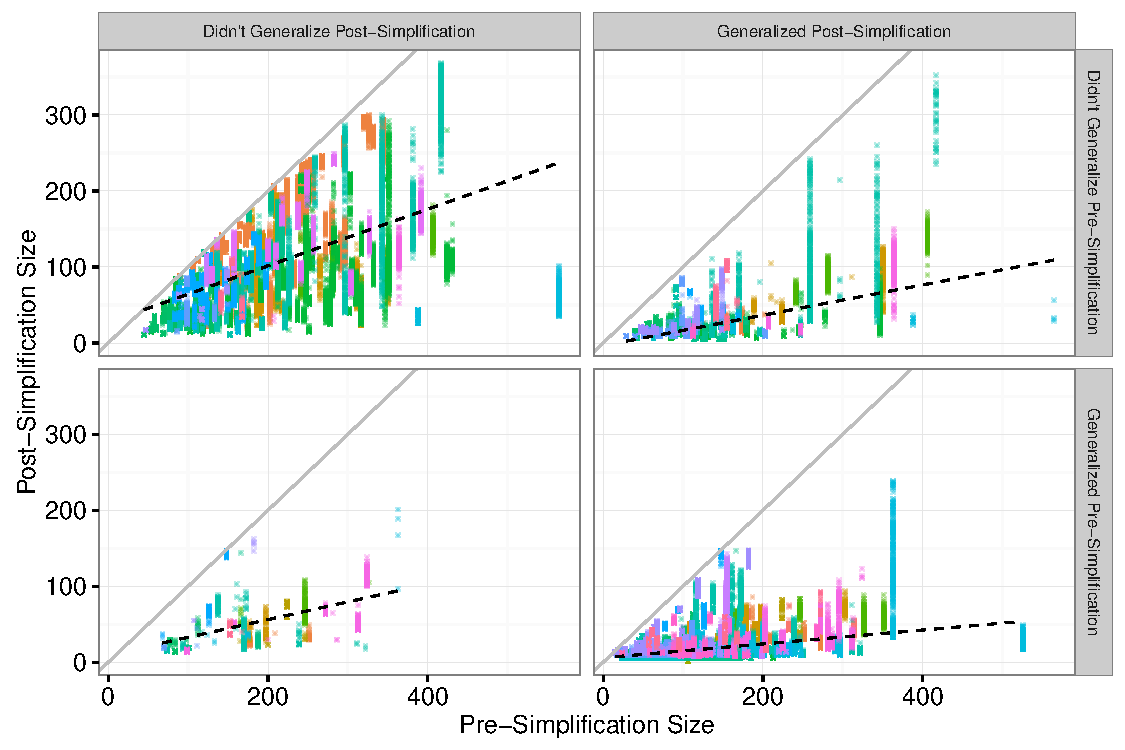
\includegraphics[width=\linewidth]{Quad_Scatter} % \linewidth
\caption{In each of the subgraphs, a simplified program is plotted at each point, with its pre-simplified size on the $x$-axis and its post-simplified size on the $y$-axis. Vertical striping is the result of simplifying each unchanged program 100 times for each of the 5 simplification methods. The top two plots contain programs that did not generalze pre-simplification, and the bottom two plots contain programs that did generalize pre-simplification. The left two plots are simplified programs that do not generalize; the right plots do generalize. For each type, we also give a linear trend line.}
\label{fig:nic-plot}
\end{figure}

In each plot we draw a linear fit line showing the relationship of unchanged size and simplified size. In the plots in the left column, in which simplified programs did not generalize, the slope is considerably higher than in the right column plots where the simplified programs do generalize. \hl{What does it mean???} \hl{This paragraph is bad and needs to be extended and edited after we see the final plot.}


%\begin{figure}[t] %[t] sets the image at the top of the page; t = top, b = bottom, h = here%
%\centering
%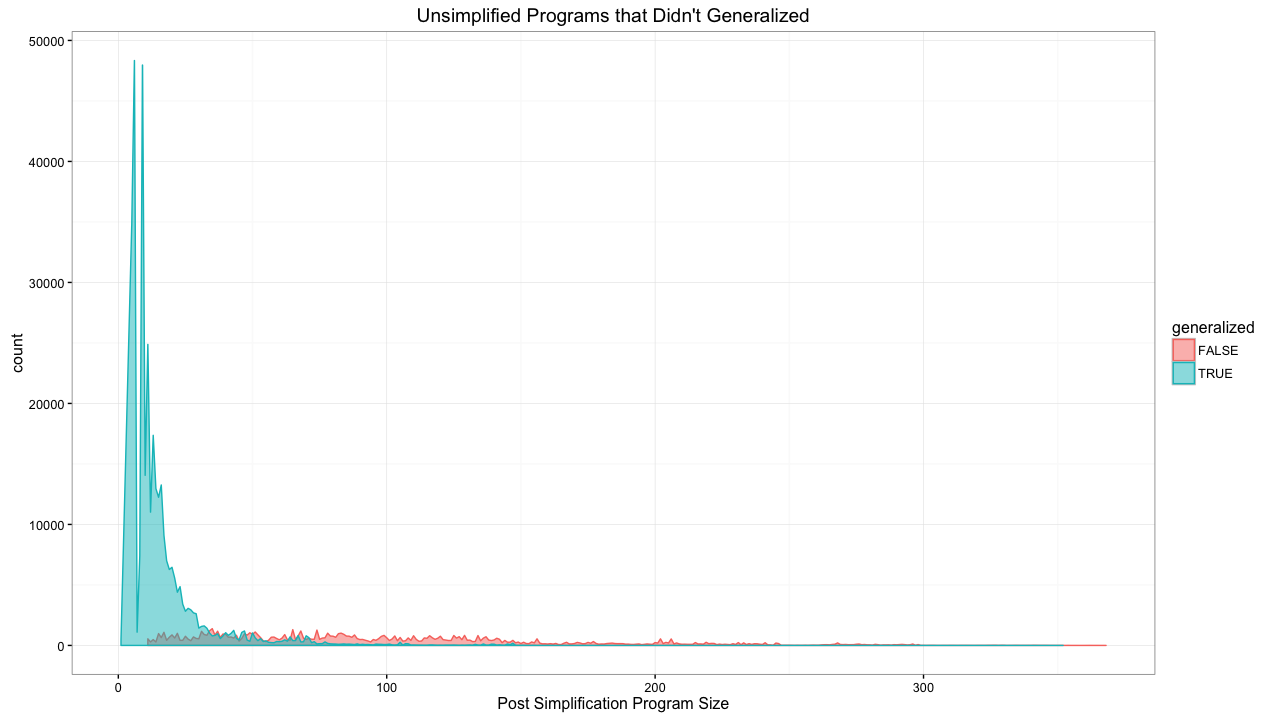
\includegraphics[width=\linewidth]{Size_density_by_generalized_count}
%\caption{Size counts of simplified programs. Includes all simplified programs, from both ones that did and did not generalize pre-simplification.}
%\label{fig:count:gen}
%\end{figure}

%These look at the same graphs, but faceted.
%
%\begin{figure}[t] %[t] sets the image at the top of the page; t = top, b = bottom, h = here%
%\centering
%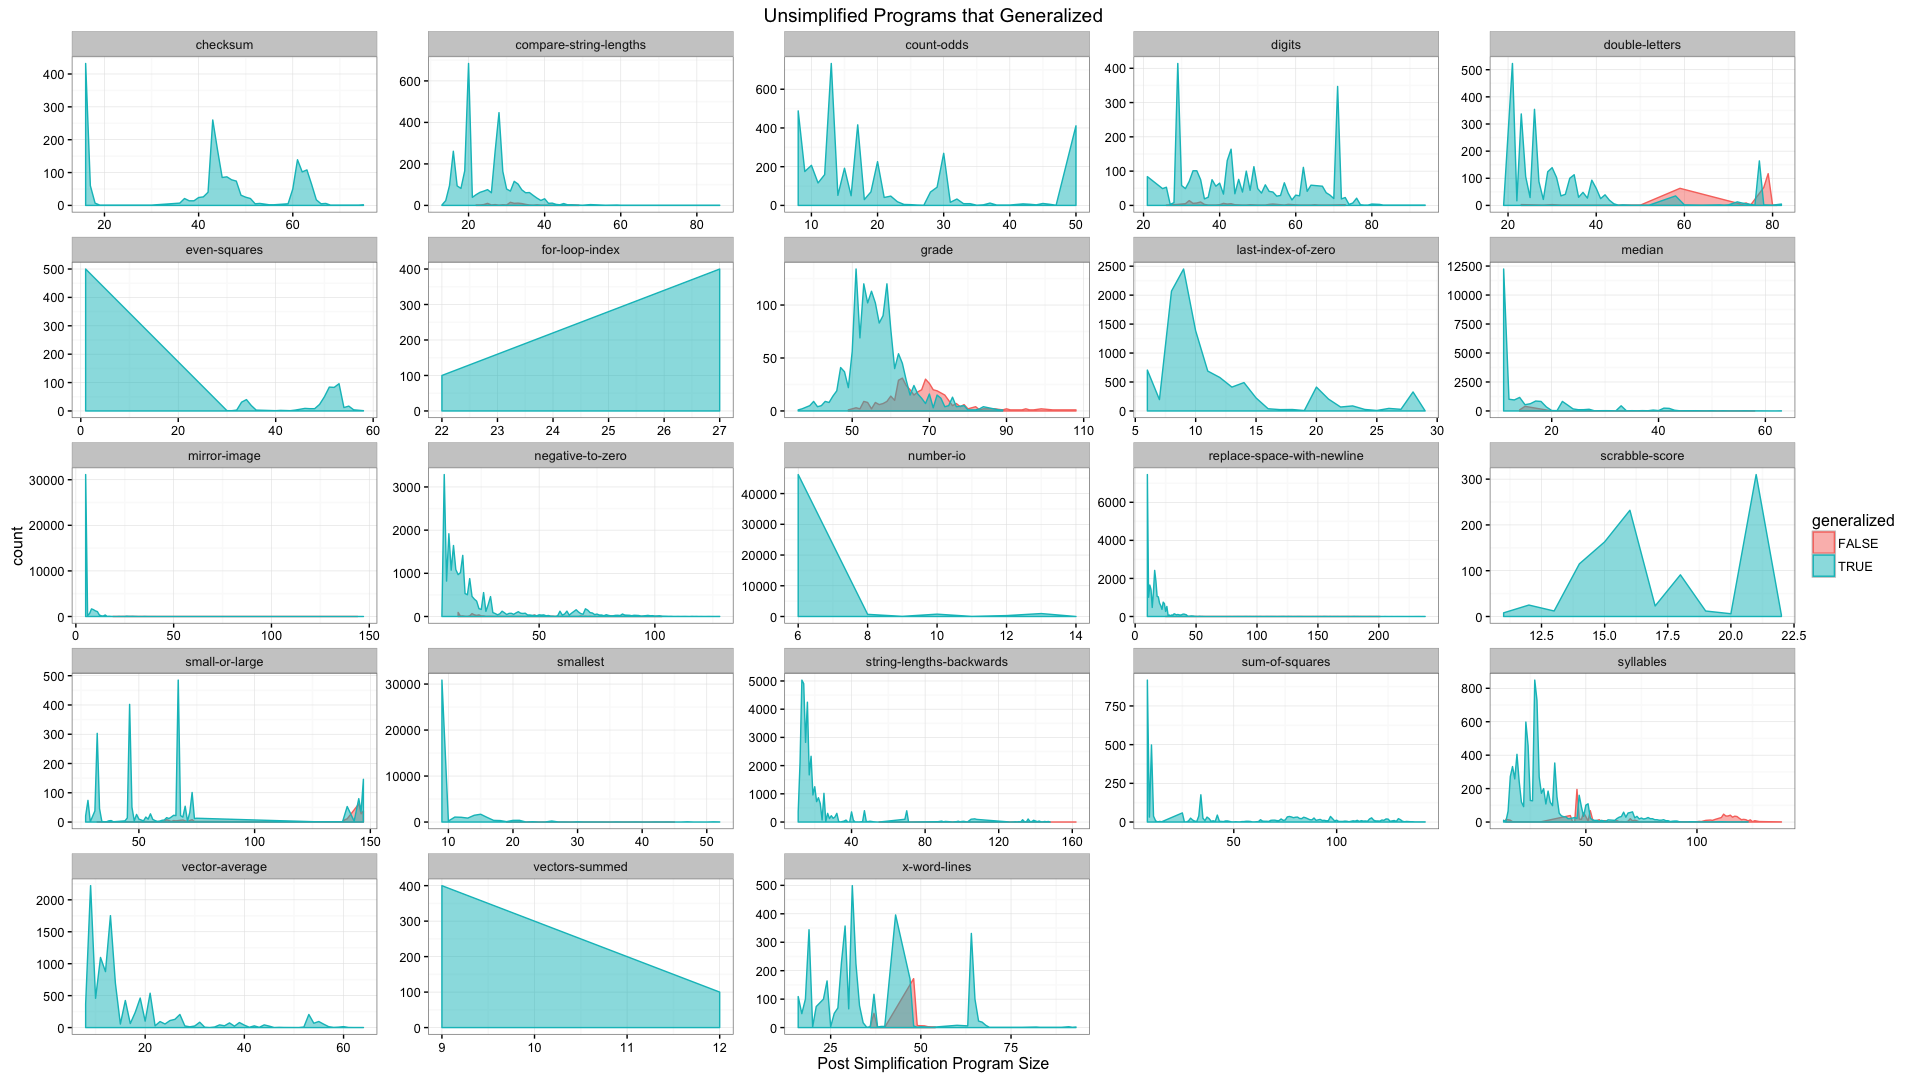
\includegraphics[width=\linewidth]{Size_density_by_generalized_A_count}
%\caption{Size counts of simplified programs where pre-simplified program did generalize.}
%\label{fig:count:pre-simp-gen-true}
%\end{figure}
%
%\begin{figure}[t] %[t] sets the image at the top of the page; t = top, b = bottom, h = here%
%\centering
%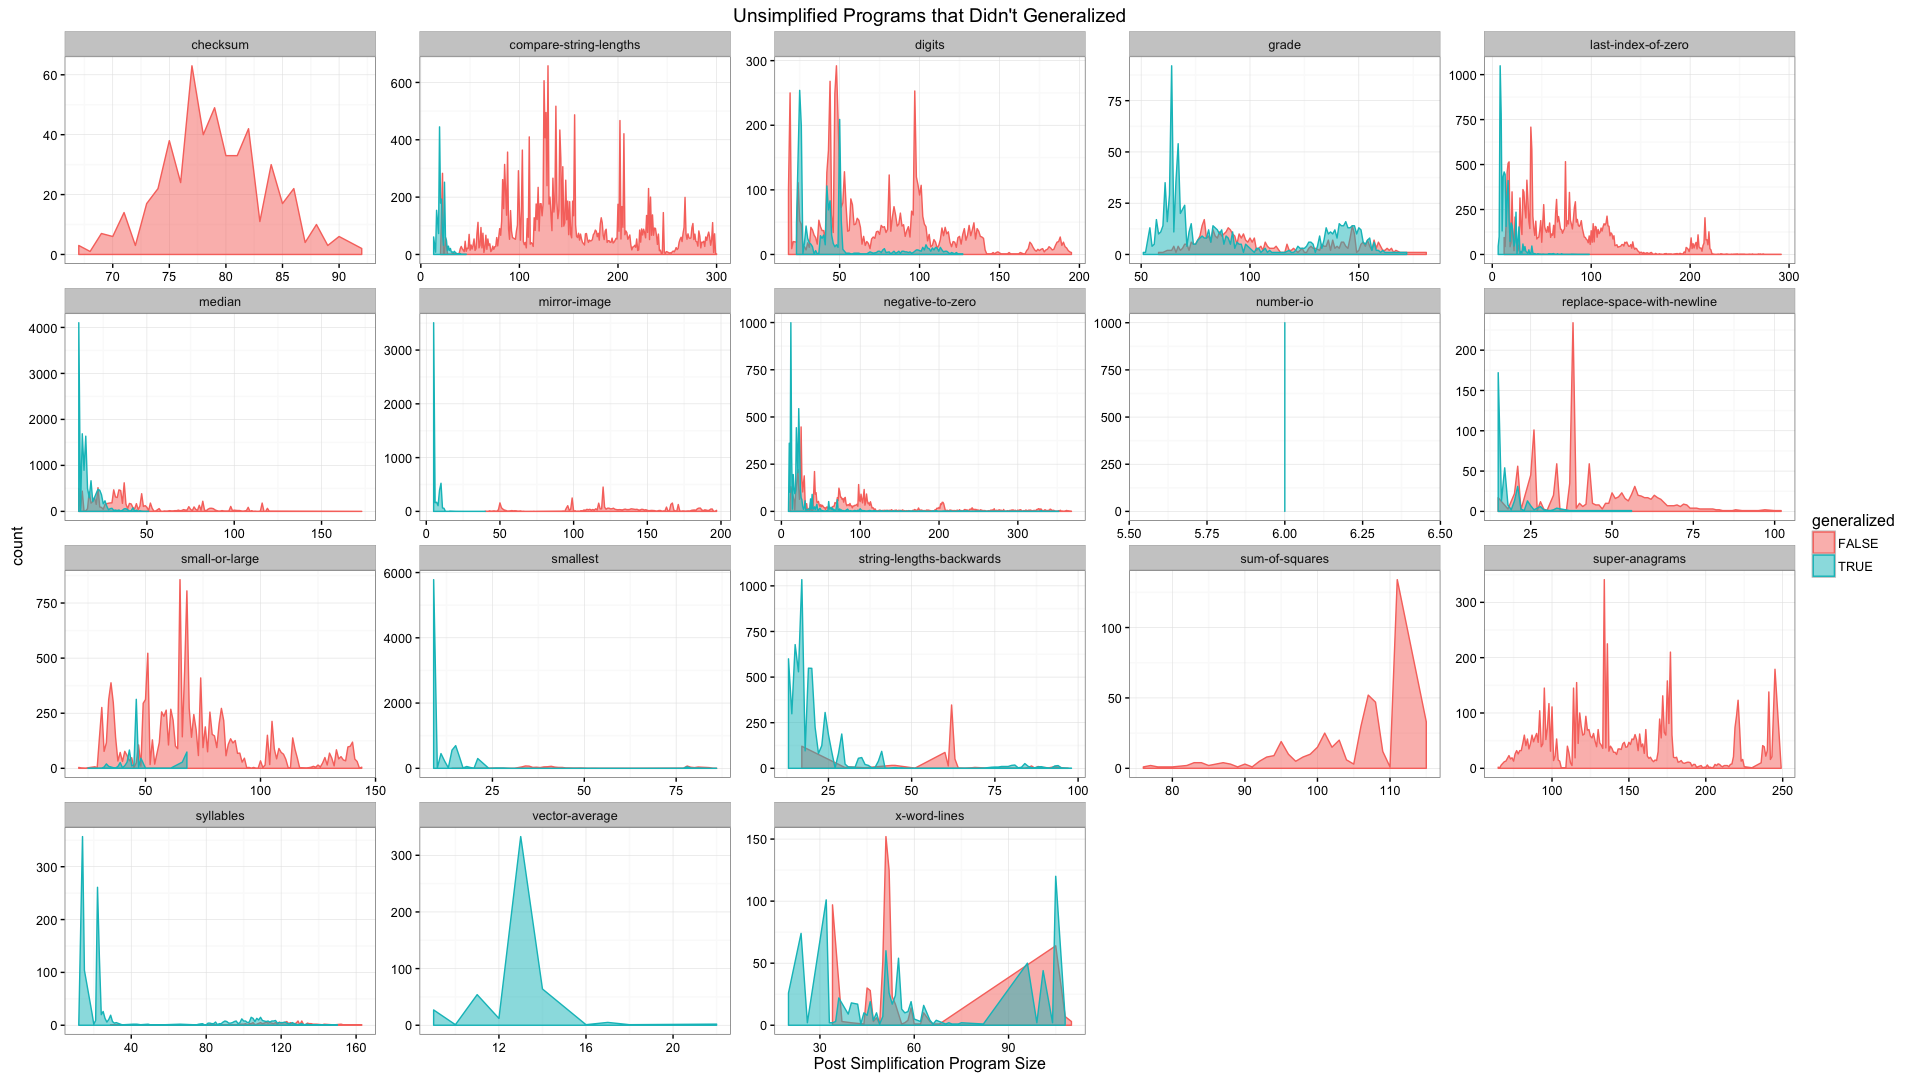
\includegraphics[width=\linewidth]{Size_density_by_generalized_B_count}
%\caption{Size counts of simplified programs where pre-simplified program did \underline{not} generalize.}
%\label{fig:count:pre-simp-gen-true}
%\end{figure}


\section{Discussion}
\label{sec:discussion}

\todo[inline]{Talk about what the results mean}

%Here are some potentially interesting questions to explore with this data:
%
%    Which simplification method tends to result in the smallest programs on average? Is there any significant differences here?
%
%    Is getting smaller during simplification important for generalization? In other words, do smaller programs post-simplification tend to generalize better than larger ones?
%
%        Note: we could ask this question of all the simplified programs, but we could also concentrate only on runs that had some generalizing programs and some non-generalizing programs, which might give us a more detailed view. It would probably be worthwhile to look into both of these. I'm not sure exactly how we would investigate this. @mcphee made some cool graphs last year that start answering this question. I've included one at the bottom of this post that was made with limited data; a similar graph for the full data might be a good place to start.
%
%    It might be worthwhile to break this big plot into smaller plots, grouping together similar plots. For example, we might group plots based on how often unsimplified programs generalize -- groups of something like 0-50\%, 50-95\%, and 95-100\% generalization. Or, we could do it some other way. But, this could definitely help with spotting differences based on problem.
%

\hl{    Would a multi-restart simplification get us to smaller programs more often than the other methods we've tried? This could potentially avoid unlucky local minima. The backtracking methods are also trying to avoid unlucky local minima, so this would be an interesting comparison. It seems like we could answer this question with the data we have.}

\todo[inline]{I don't really see how we could answer that question with
this data? It's definitely a cool question, but seems more future work
than this paper. -- Nic}

As noted earlier, all five simplification methods lead to substantial
reductions in program size across all 24 test problems, as shown in
Figure~\ref{fig:bar:size}, with the average simplified sizes often 
well under half the original sizes, and sometimes much smaller than that.

Further, all the simplification methods improved generalization rates for
all but a few problems (see Figure~\ref{fig:bar:percent_generalization}),
but again with little difference among the simplification methods.
In some cases, e.g., count-odds, all the unsimplified programs already
generalized, so the best simplification could do is to not make things
worse. In other cases, such as
checksum, double-letters, and vectors-summed, there were very few 
solution programs generated in the initial 100 PushGP runs (5, 6, and 1,
respectively). With so few data points to work with it's not surprising
that in some cases (e.g., checksum and vectors-summed) there was no change
in generalization. In the case of double-letters, five of the six initial
solutions were consistently simplified without affecting generalization.
The sixth solution, however, frequently let to simplifications that no 
longer generalized. Only 37 of the 100 Program simplification results, 
for example, generalized, while only 45 of the 100 Genome simplifications
generalized.

\todo[inline]{All the the failures I've looked at (and I looked at quite a
	few) have a total error of 6, with errors of 2 on the same three test
	cases. They all share a weird sequence of 20 `!' characters in a row
	early in their simplified programs, which smells really fragile to me,
	but I haven't dug into the programs enough to know if that's the issue.}

It's also clear from Figures~\ref{fig:count:quad} and~\ref{fig:nic-plot} that
smaller post-simplification sizes were strongly correlated with the
ability to generalize after simplification. This is consistent with 
a broad range of work that either argues theoretically (e.g., the minimum
description length principle~\cite{iba1994genetic, zhang1995balancing}) 
and/or empirically
that smaller programs will be more likely to generalize~\cite{thing1, thing2}.
While there have been contrary results that show that program size and
generalization are not always correlated~\cite{silva2012operator}, the
correlation seems extremely strong in our data. 

The relationship between
program size and generalization is almost certainly driven at least in part
by both the problem being solved, and the representation being used for
solutions. It's possible, therefore, that the strong correlation we see
is in some way related to the kinds of software synthesis problems we're using
as benchmarks, which clearly behave differently from the commonly used
symbolic regression and classification benchmarks. 

It's also possible,
however, that the design decisions in PushGP play a crucial role here. Any
attempt to control or reduce program size in GP is premised on the idea that
there must be some parts of the program that aren't playing an important role
and can thus be removed; such code has been called many things over the years,
such as ``introns'' or ``bloat''. The fact that the evolved PushGP solutions
were bigger than strictly necessary (often by a substantial margin) is arguably
not attributable to ``bloat'' as it's typically been 
understood~\cite{poli08:fieldguide}, since in PushGP we don't see a 
general tendency towards increasing program size over time. 

There is obviously ``unnecessary'' code in these evolved Push programs, 
however, but Understanding the source and role of this removable Push 
code is complex, in part because there are potentially many categories 
of ``unused'' or ``unnecessary'' code
in Push. Examples include:
\begin{itemize}
	\item Instructions that do nothing because they require arguments 
	that aren't on the appropriate stacks when they're executed. 
	\item Instructions that do \emph{something}, but not something that has an 
	impact on the final result because, e.g., they act on values on stacks 
	that play no role in the key computation. 
	\item Instructions whose \emph{presence} is important (e.g., as a marker 
	or to make sure the \texttt{exec} stack has the right size), but 
	whose details or \emph{behavior} isn't.
\end{itemize}
Note also that the ``activity'' of many of these instructions is highly
dependent on context. An instruction that does nothing in a parent because
the arguments it needs aren't available, might play a prominent role in a
child if a change ``upstream'' causes those arguments to now be available.

These dynamics are very different from many tree-based GP systems, where
changes in argument subtrees will change the \emph{value} computed at a 
node, but won't typically change the \emph{semantics} of the operator at that
node. A plus node in a tree will always do addition, even if changes in its
arguments lead to different sums; the plus node will (in most tree-based
systems) never simply fail to act because an argument is missing.

So in the same way that the design of our simplification methods was
tightly coupled to the details of Push and Plush, it would not be surprising
if at least some of the results (e.g., the relationship between size and
generalization) were also tied to the specifics of PushGP. One common
anecdotal observation is that unsimplified evolved Push programs often
contain large numbers of looping and recursion constructs that are removed
in the simplification process. It's possible that in many cases these loops
are performing ``unnecessary'' computation and counting on the PushGP
execution limits to stop them and force the return of an answer. This sort
of approach is likely to be quite brittle, and eliminating these unnecessary
loops might be a source of improved generalization. All of which is rather
deeply intertwined with key details of PushGP.

\todo[inline]{We should grab an empirical citation or two about small
programs generalizing better. The Silva GPEM paper~\cite{silva2012operator}
would probably be a good place to do some digging.}

\subsection{Nic's Thoughts on Unused Push Instructions}
\hl{Anyway, I wouldn't recommend using the word ``bloat'' because I also think that is generally associated with a tendency to get bigger and bigger and bigger in ways that aren't connected to improvements in fitness, and that doesn't seem to be a Clojush thing. (I'm personally not super clear on why that's not a thing in Clojush, etc., etc., but that's not today's problem.)

Even more complicated is the fact that in Push programs we often find various categories of ``unused'' code. There are instructions that do nothing because their arguments aren't on the stack, or sometimes aren't on the stack. There are instructions that do something, but no one cares (they push a boolean that's never used). There are instructions that are there just to add content to a stack, but who's particular action doesn't matter. Etc., etc. These are not things ``standard tree-based GP'' people run into very often, and might not be obvious to them.

Lastly, it can be really hard to tell what's being used and how in complex programs, and how that relates to the simplified versions. It's easy to implicitly assume that the simplified program is ``the thing'', and that everything that got removed didn't really matter in the original execution. (This is often an assumption in tree-based bloat discussions.) I'm pretty sure this is often very not true, however, in Push, and that's important to the generalization. It seems fairly common, for example, for Push programs (especially with the ``standard'' instruction set) to have a lot of unnecessary looping that frequently gets removed or reduced in simplification. Often that looping is actually executed in the original program, so it's part of how the training answers are formed. I have a suspicion that part of why simplification often improves generalization is that it removes these unnecessary loops that are sometimes fragile and do weird things on certain inputs.}



\section{Related Work}
\label{sec:related}

\todo[inline]{Tom: I'm fine moving this section earlier if others prefer.}

\todo[inline]{Below are things I've (Tom) come across in the past year potentially realted to this work. We'll have to go through and see what's worth citing.}

\subsection{Papers about automatic simplification}

\begin{itemize}

\item
Genprog minimization after run (see 7/24/16)

\item
Field Guide to Genetic Programming: p 64 top: Bahnzaf paper might be precursor to automatic simplification

\item
This paper in neural networks might be related: GECCO 2016 - Identifying Core Functional Networks and Functional Modules within Artificial Neural Networks via Subsets Regression

\item
Differentiate between our work and algebraic simplification (as used in semantic GP), since this CAN change the semantics on inputs not in the training set, where algebraic methods cannot. Also, algebraic methods wouldn't work on general programs that we're evolving

\item
Algebraic Simplification of GP Programs During Evolution (I think this is an actual paper title)

\item
Investigation of simplification threshold and noise level of input data in numerical simplification of genetic programs \cite{Kinzett:2010:cec}

\item
Smaller networks in neural nets: https://push-language.hampshire.edu/t/gecco-2017-simplification-for-generalization/660/21?u=thelmuth

\end{itemize}

\subsection{Papers about generalization and overfitting in GP}

\begin{itemize}
\item
GECCO 2011 - Variance based Selection to Improve Test Set Performance in Genetic Programming

\item
Controlling overfitting in symbolic regression based on a bias/variance error decomposition


\end{itemize}

\subsection{Other related papers}

\begin{itemize}
\item
Tree-structured differencing: R. Al-Ekram, A. Adma, and O. Baysal. diffX: an algorithm to detect changes in multi-version XML documents. In Conference of the Centre for Advanced Studies on Collaborative research, pages 1–11. IBM Press, 2005.

\item
Delta debugging: A. Zeller. Yesterday, my program worked. Today, it does not. Why? In Foundations of Software Engineering, pages 253–267, 1999.

\end{itemize}

\section{Conclusions and future work}
\label{sec:conclusions}

\todo[inline]{Maybe this could/should be two sections, but I bet we won't have room.}

FUTURE WORK BELOW HERE

Testing automatic simplification on other types of problems. Would it work on symbolic regression? Classification? My (TMH) guess is that it would work better on classification than symbolic regression.

How could simplification be adapted for tree-based GP? How about other GP, such as Cartesian or grammar-based? Grammatical evolution could potentially remove numbers from the genome, or could replace trees in the resulting program. Other linear GPs seem like good targets.

\begin{acks}
  
  \todo[inline]{Put acknowledgements here, including grants.}

\end{acks}
